\documentclass[12pt]{article}
\usepackage[english]{babel}
\usepackage[utf8]{inputenc}

\usepackage{geometry}
\geometry{
	letterpaper, 
	portrait, 
	top=.75in,
	left=.8in,
	right=.75in,
	bottom=.5in		} 	% Page Margins
	
%% additional packages for nice things
\usepackage{amsmath} 	% for most math
\usepackage{commath} 	% for abs
\usepackage{lastpage}	% for page count
\usepackage{amssymb} 	% for therefore
\usepackage{graphicx} 	% for image handling
\usepackage{wrapfig} 	% wrap figures
\usepackage[none]{hyphenat} % for no hyphenations
\usepackage{booktabs} 	% enhanced table qualities
\usepackage{array} 		% for >{} column characterisctis
\usepackage{physics} 	% for easier derivative \dv....
\usepackage{tikz} 		% for graphic@!
\usepackage{circuitikz} % for circuits!
\usetikzlibrary{arrows.meta} % for loads
\usepackage[thicklines]{cancel}	% for cancels
\usepackage{xcolor}		% for color cancels
\usepackage[per-mode=fraction]{siunitx} % for si units and num
\usepackage{fancyhdr} 	% for header
\usepackage{comment}	% for ability to comment out large sections
\usepackage{multicol}	% for multiple columns using multicols
\usepackage[framed,numbered]{matlab-prettifier} % matlab sytle listing
\usepackage{marvosym} 	% for boltsymbol lightning
\usepackage{pdflscape} 	% for various landscape pages in portrait docs.
\usepackage{float}
\usepackage{fancyvrb}	% for Verbatim (a tab respecting verbatim)
\usepackage{enumitem}	% for [resume] functionality of enumerate

%% package config 
\sisetup{output-exponent-marker=\ensuremath{\mathrm{E}}} % for engineer E
\renewcommand{\CancelColor}{\color{red}}	% for color cancels
\lstset{aboveskip=2pt,belowskip=2pt} % for more compact table
\def\arraystretch{1.4} % adjust size of arrays
%\arraycolsep=1.4pt\def
\setlength{\parindent}{0cm} % Remove indentation from paragraphs
\setlength{\columnsep}{0.5cm}
\lstset{
	style      = Matlab-editor,
	basicstyle = \ttfamily\footnotesize, % if you want to use Courier - not really used?
}
\renewcommand*{\pd}[3][]{\ensuremath{\dfrac{\partial^{#1} #2}{\partial #3}}} % for larger pd fracs
\renewcommand{\real}[1]{\mathbb{R}\left\{ #1 \right\}}	% for REAL symbol
\newcommand{\imag}[1]{\mathbb{I}\left\{ #1 \right\}}	% for IMAG symbol
\definecolor{m}{rgb}{1,0,1}	% for MATLAB matching magenta
	
%% custom macros
\newcommand\numberthis{\addtocounter{equation}{1}\tag{\theequation}} % for simple \numberthis command
\newcommand{\equal}{=} % so circuitikz can have an = in the labels
\newcolumntype{L}[1]{>{\raggedright\let\newline\\\arraybackslash\hspace{0pt}}m{#1}}
\newcolumntype{C}[1]{>{\centering\let\newline\\\arraybackslash\hspace{0pt}}m{#1}}
\newcolumntype{R}[1]{>{\raggedleft\let\newline\\\arraybackslash\hspace{0pt}}m{#1}}

%% Header
\pagestyle{fancy} % for header stuffs
\fancyhf{}
\rhead{Thad Haines \\ Page \thepage\ of \pageref{LastPage}}
\chead{Talking Points \\ Week of May 20th, 2019}
\lhead{Research \\ }
% spacing
\headheight 29 pt
\headsep 6 pt

\begin{document}
\begin{multicols}{2}

	\paragraph{Recent Progress:}
	\begin{enumerate}
		\item MiniWECC step test results using different time steps (see reverse).
		
		\item Matt approach of ggov1 model attempted.

		\item Code flowchart being compiled to aid in further development (timing).

		\item Shunts and Branches added to Mirror
		\item custom \verb|single2float| function added to reduce casting error during PSLF$\longrightarrow$LTD value exchange

		\item \verb|shelve|, instead of \verb|pickle|, used for python data storage. Leads to more consistent read/write operations.

	%	\item More \verb|matplotlib| plot functions created.

		\item GitHub updated:\\
		\verb|https://github.com/thadhaines/PSLTDSim/|
		
	\end{enumerate}
\paragraph{Current Tasks:}
	\begin{enumerate}
		\item Add logging to Shunt and Branch Agents
		\item Add perturbance Agents for Generator/Slack, Shunt, Branch, \ldots
		\item Formulate feasible plan of action for casting all WECC governors to LTD governors (tgov1). Something like:
		\begin{enumerate}
		\item Parse models of interest from dyd.
		\item Automate one machine infinite bus test in PSDS.
		\item Generate/Calculate LTD equivalent model parameters from results
		\item Export custom dyd for LTD simulation. (PSDS would still use original the dyd, though \emph{could} use modified dyd)
		\end{enumerate}
		
		\item Create an agent for every object: \\ SVD, Transformer, \ldots

		\item Define Agent actions for \\ AGC/LFC (i.e. ACE calculations)
		%\subitem A FlowtabrDAO exists that can find flow between busses. A way to initialize bus connections between areas has yet to be devised.
		

	\end{enumerate}
%\pagebreak
\vfill\null
\columnbreak

\paragraph{Future Tasks:}(Little to No Progress since last time / Things coming down the pipe)
	\begin{enumerate}

		\item Formulate an experiment utilizing a multi-area model that can be validated with PSDS.
		\item Revisit tgov1 model to account for \verb|LoadRef| / \verb|Pref|.
		\item Investigate line current data and ULTC action in PSLF.
		\item Think about Shunt Control / Generic Agent control based on system state(s)

		\item Add import mirror / bypass mirror init sequence option. Will prevent repeated WECC mirror creations.

		\item Identify System Slack bus programmatically (currently assumes first slack == global slack if > 1 slack found)
		\subitem AND/OR calculate system slack error differently $\rightarrow$ An average of slack errors?

		\item Matt request: Enable multiple dyd files to overwrite / replace previously defined agents/parameters
		
		%\subitem Can locate when only 1 Slack exists. If more than one Slack, maybe identify by generator with most busses under control? Proving more difficult than expected. Can identify in PSLF via the \verb|summ()| or \verb|isld()| commands. 
		
	\end{enumerate}
	\paragraph{Current Questions:}
	\begin{enumerate}
		\item Overview of planned PSLF scenarios? $\rightarrow$ Similar to Heredia paper but on Wecc/MiniWecc Scale? 
		
		\item Is there more available/relevant event data that may help us to verify simulations of specific instances (wind ramps or other behavior) that novel research will focus on? %(Heredia paper data helpful for some wind ramp data context)

		\item  Any progress / continued interest in miniWecc Area definitions?

	%	\item Any progress on Wecc single gen per bus system?
	%	\\ Will this actually matter? PSLF handles distribution of Pe in power flow solution per bus, and LTD code distributes electrical power per generator... Voltage issues maybe, but power should be okay.
		
		
%		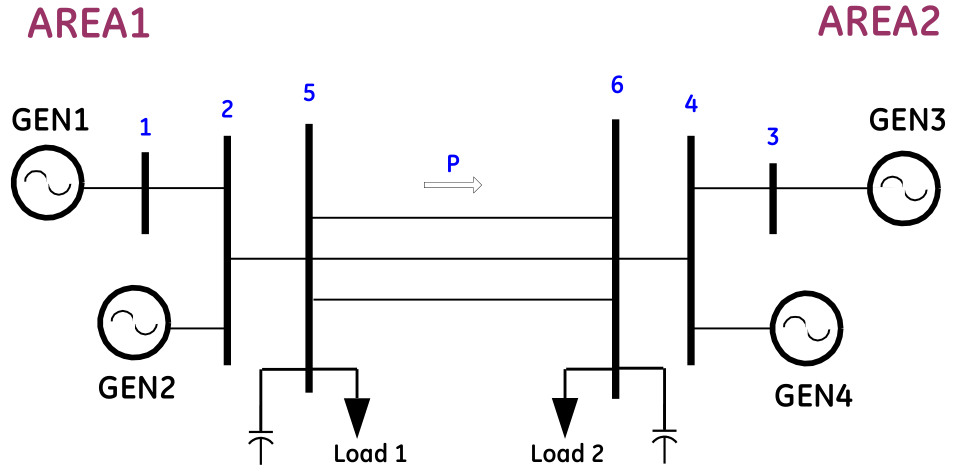
\includegraphics[width=\linewidth]{g4aSys}
	\end{enumerate}
\paragraph{Goals:}
	\begin{enumerate}
	\item Speed$\longrightarrow$ Order of Magnitude faster than PSDS (not met --- only $\approx$2x faster)
	\end{enumerate}

\vfill\null

\end{multicols}
\pagebreak
\paragraph{Time step resolution:} Changing the time step affects accuracy, size of data collected, and simulation run time. The following data was collected from a 90 second MiniWECC simulation. LTD is ran from the command line and uses rk45 integration and 0.5 MW slack tolerance.The PSDS system simulates exciters and PSS. (PSDS produces a .chf, LTD produced a .mir)

\begin{table}[!ht]
	\centering
	\footnotesize % this will affect the table font (makse it 10pt)
	\begin{tabular}{@{} lrrrrrrr @{}} 	
		\toprule % @ signs to remove extra L R space
		  & Time step  & \shortstack{Simulation\\ Time [sec] } & \shortstack{Data File \\Size [KB] }  & \shortstack{Real time \\Speed up}& \shortstack{ PSDS\\Speed up} & \shortstack{Reduction \\ of file size}  & \shortstack{Steady State $f$ \\ varience [Hz]}\\
		\midrule		
		PSDS	& 4.167 ms &  56.12   & 35,070 & 1.60& 1 & 1 & 0\\
		LTD		&	2 sec	& 13.79   &	238 &6.53&4.07 & 147.35 & NA \\ % miniWECC_loadStep01F.mir
		LTD		&	1 sec	& 27.22   &	479 &3.31&2.06 & 73.21& 9.50E-4\\ % miniWECC_loadStep02F.mir
		LTD		&	0.5 sec	& 53.56   &	871 &1.68&1.05 & 40.26 & 9.71E-4\\ % miniWECC_loadStep03F.mir
		LTD		&	0.25 sec	& 104.76   &	1,655 &0.86&0.54 & 21.19& 9.77E-4\\ % miniWECC_loadStep04F.mir
		\bottomrule
	\end{tabular}
\end{table} 
\vspace{-1em}
	\begin{figure}[h!]
			\centering
			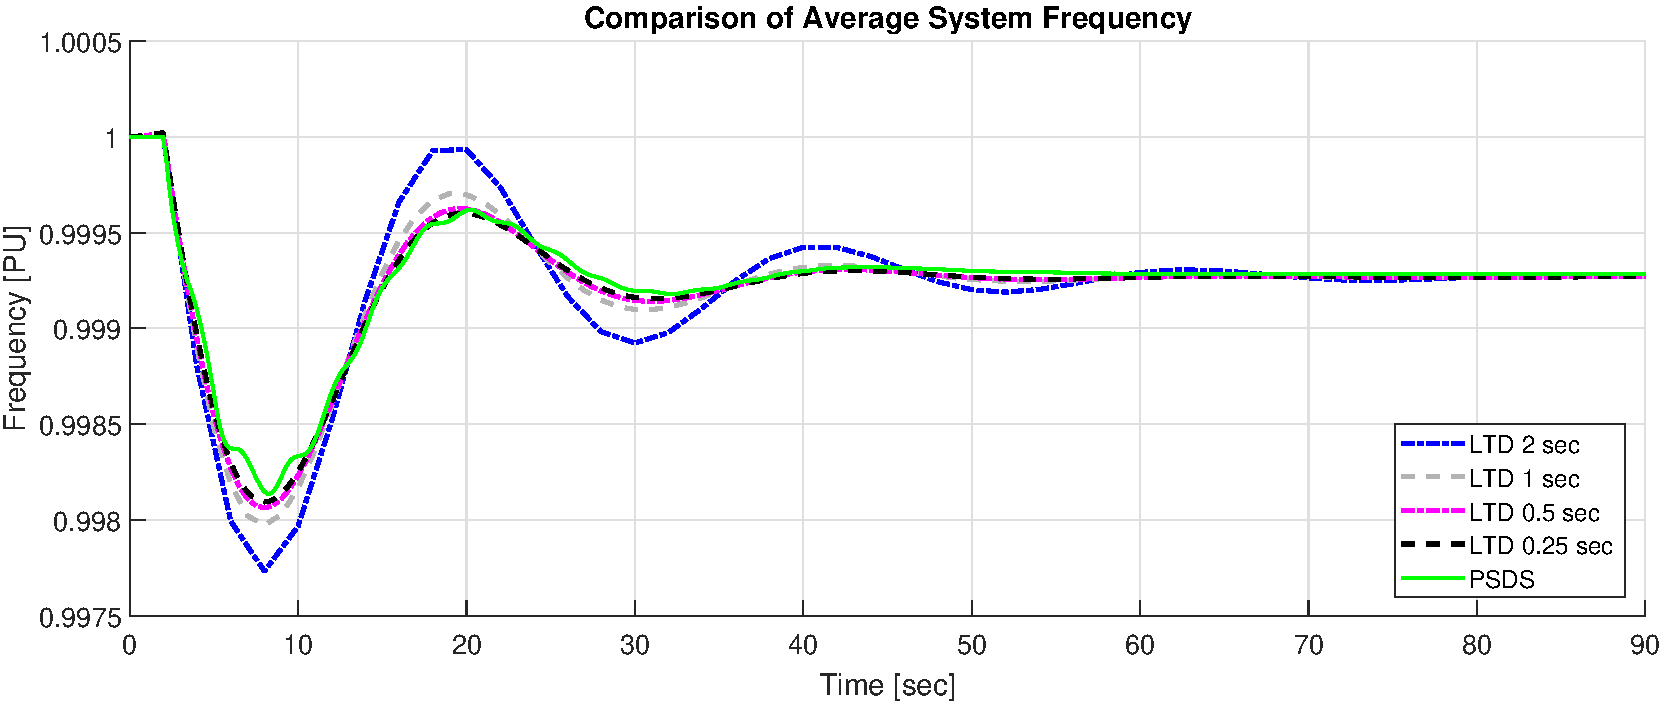
\includegraphics[width=\linewidth]{tsComp}\vspace{-1em}
			\caption{System frequency among different time steps during a 1,200 MW load step.}
			\label{tsComp}		 
	\end{figure}\vspace{-.5em}

	\begin{figure}[h!]
			\centering
			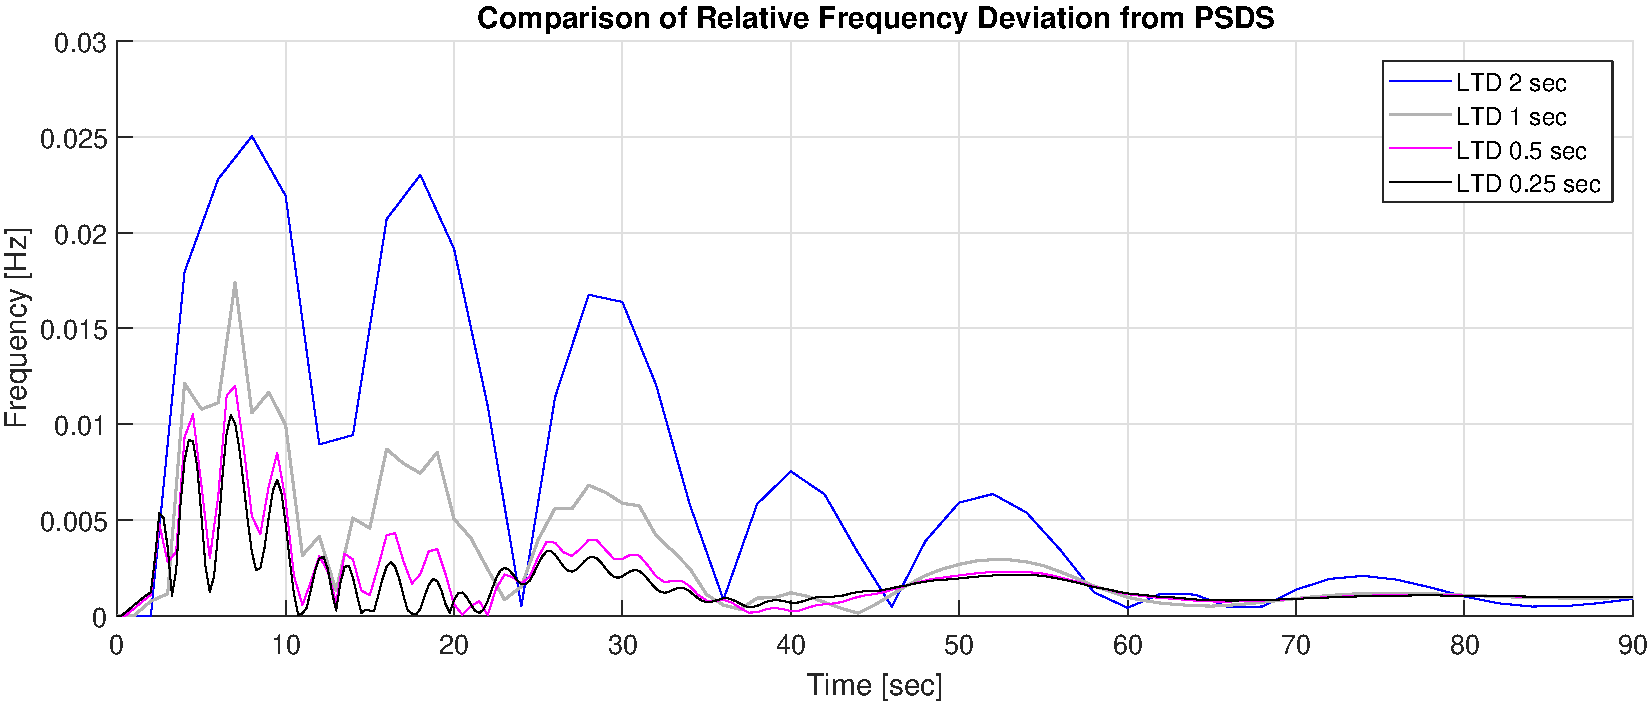
\includegraphics[width=\linewidth]{tsCompRelF}\vspace{-1em}
			\caption{Relative Hz difference of PSDS - LTD $\left( \text{i.e. }  \left|f_{PSDS}(t)- f_{LTD}(t)\right| \times 60 \text{Hz} \right)$.}
			\label{tsComp}		 
	\end{figure}\vspace{-.5em}

\begin{comment}
\pagebreak
\vspace{-1em}
	\begin{figure}[ht!]
	\begin{center}
		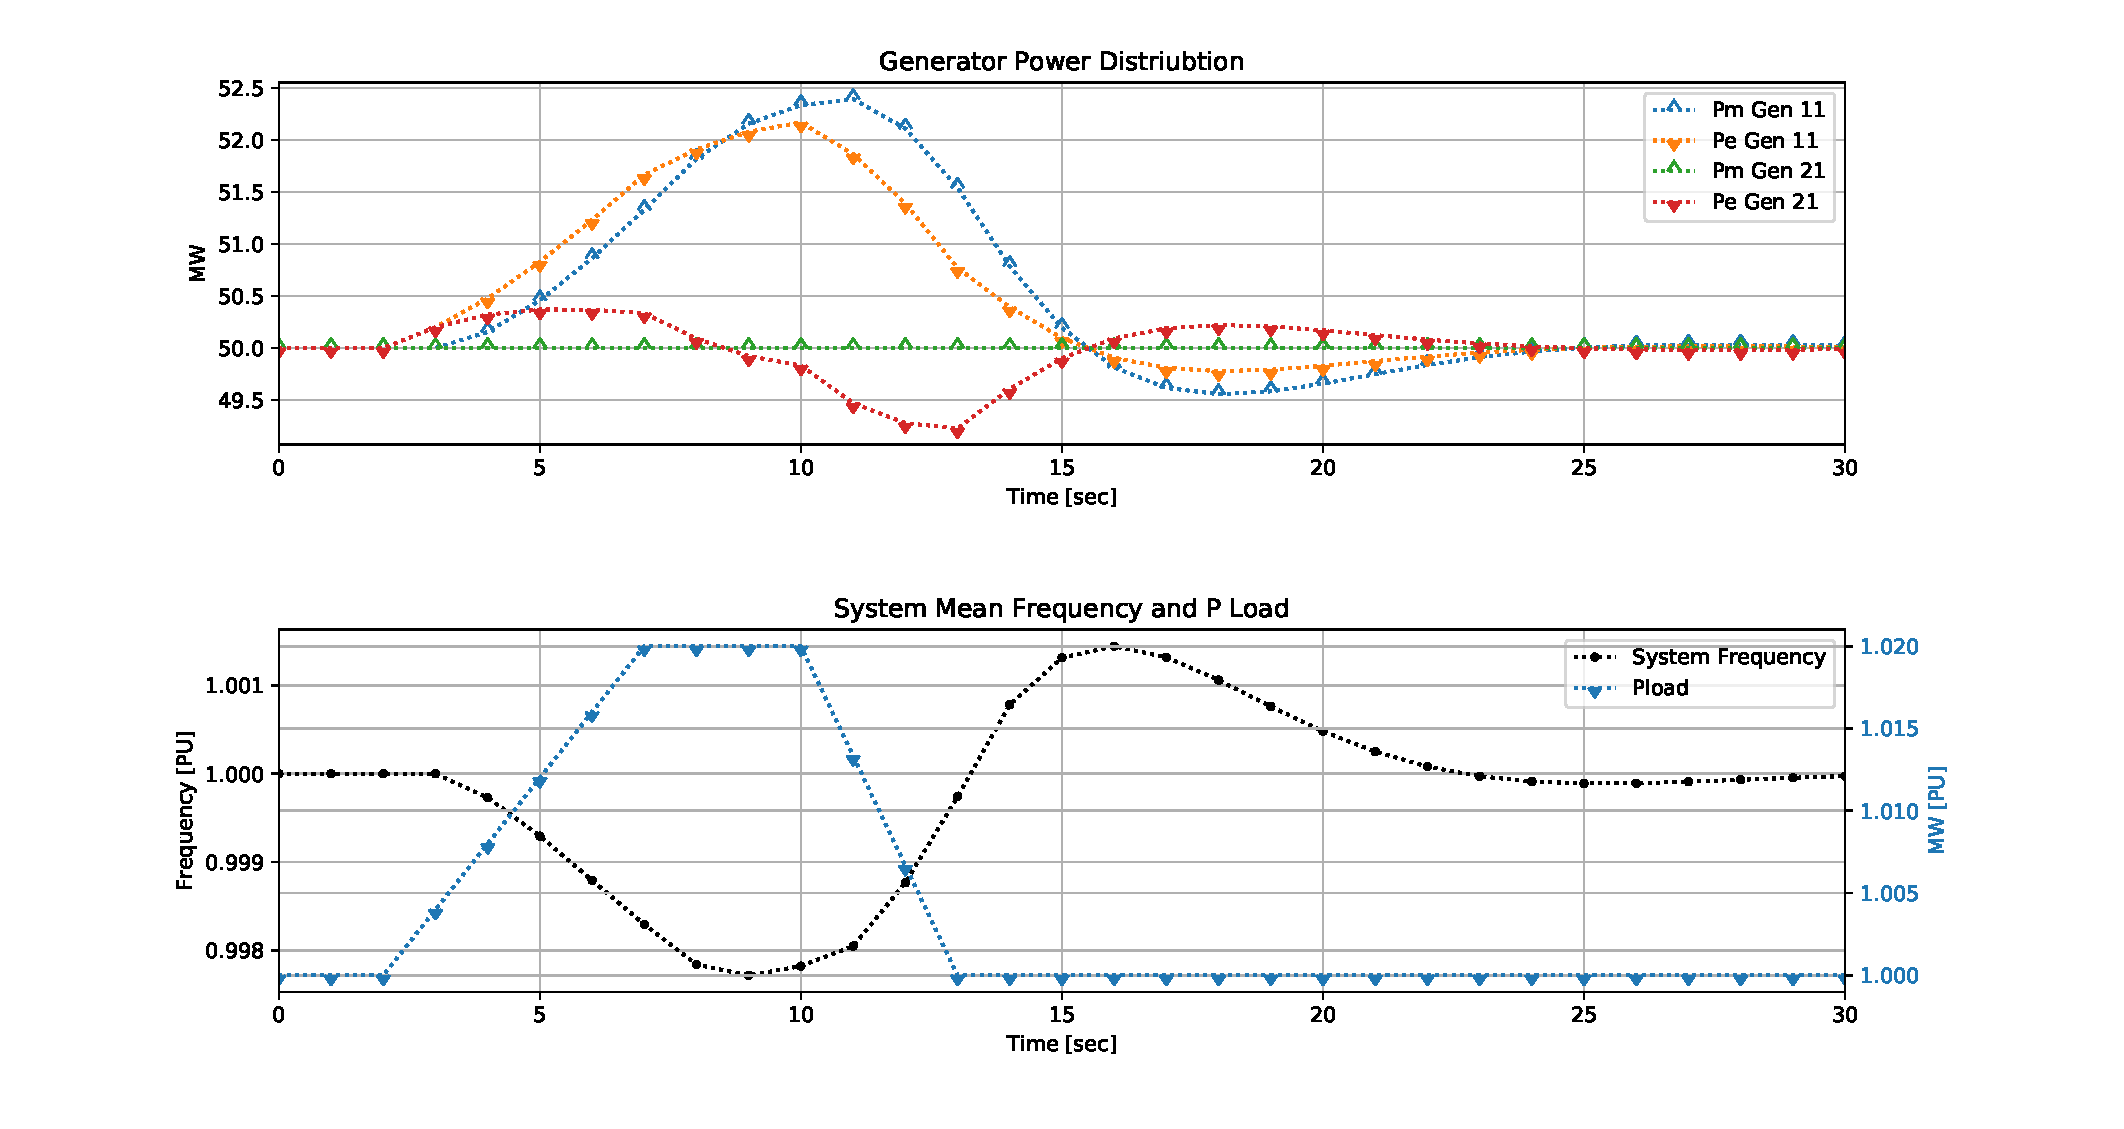
\includegraphics[width=.9\linewidth]{PY3ramp1sec}  \vspace{-2em}
		\caption{Python Ramp Simulation Single tgov1 Output - 1.0 second time step}
		\label{2gov1}\vspace{1.em}
		
		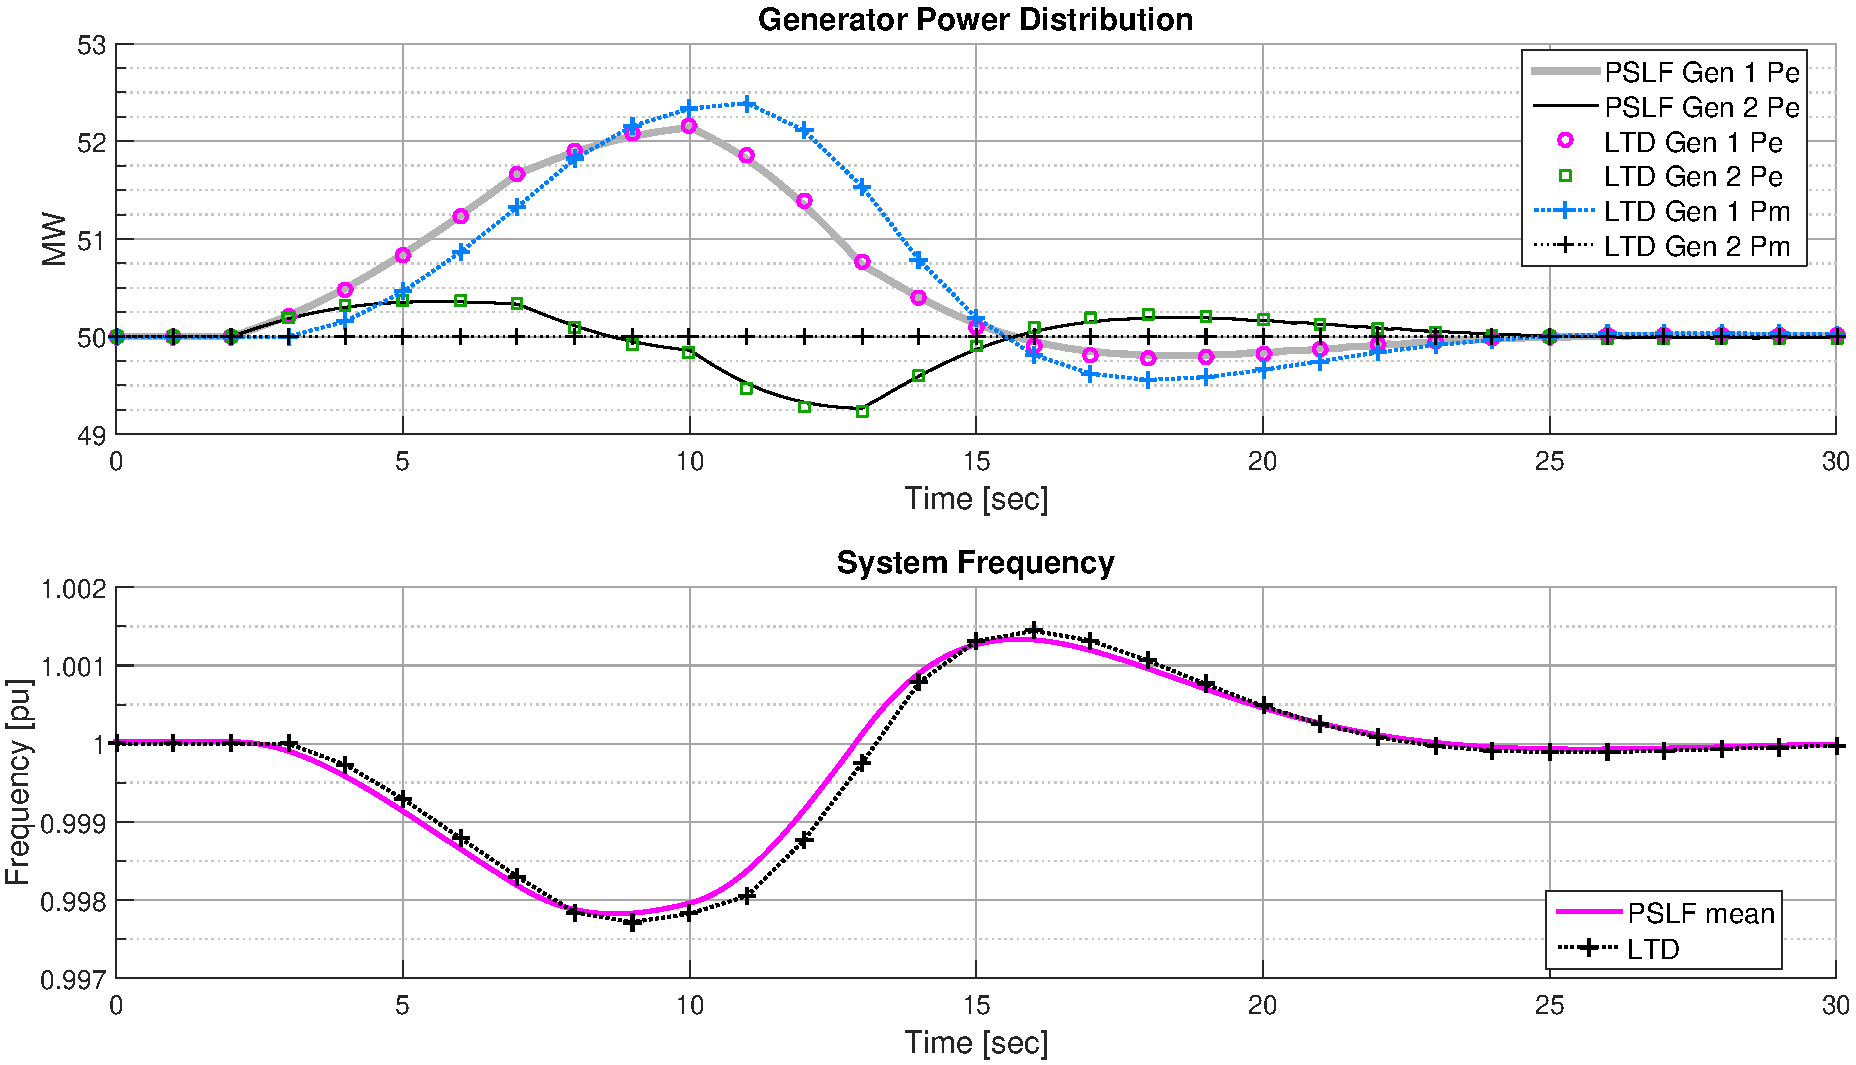
\includegraphics[width=.75\linewidth]{ramp1sec}  \vspace{-1em}
		\caption{Ramp Simulation Comparison - Single Governor - 1.0 second time step}
		\label{2gov2}\vspace{1.em}
		
		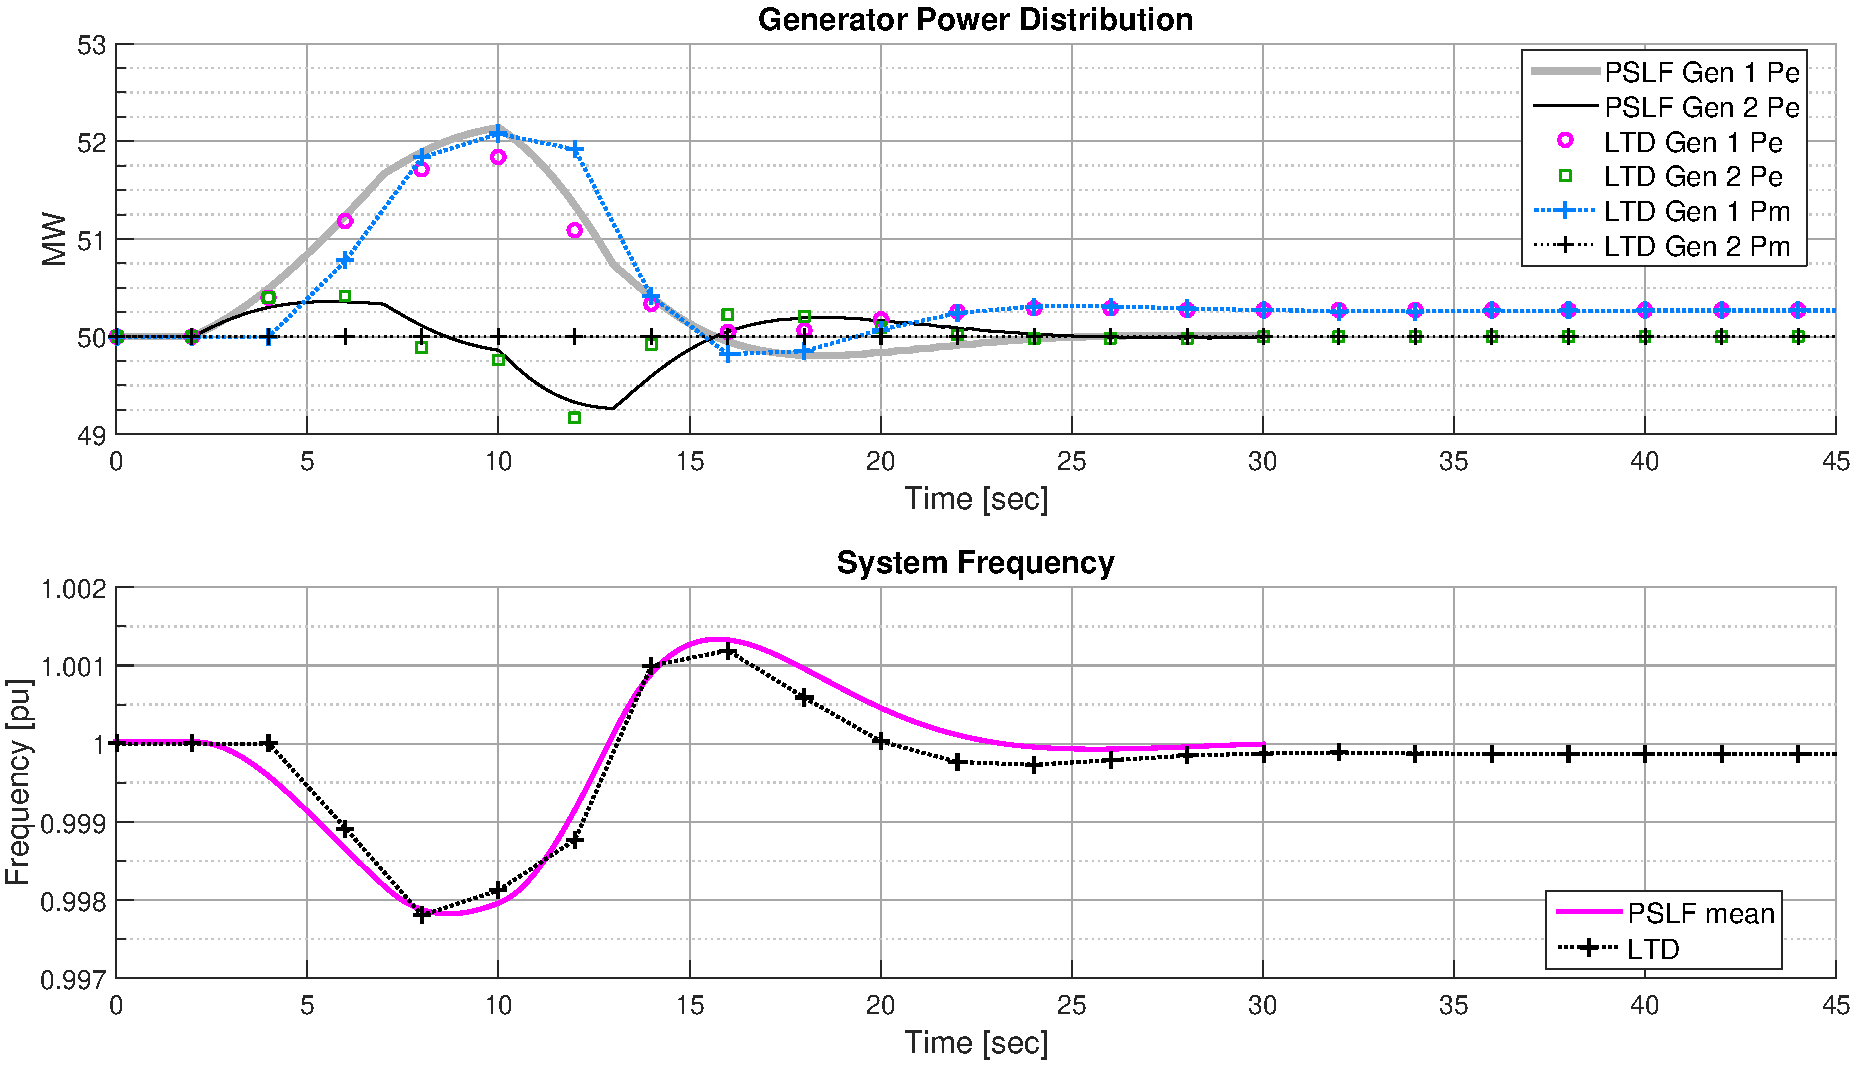
\includegraphics[width=.75\linewidth]{ramp2sec}  \vspace{-1em}
		\caption{Ramp Simulation Comparison - Single Governor - 2.0 second time step}
		\label{2gov3}\vspace{1em}
	\end{center}
\end{figure}


\pagebreak

\begin{landscape}
\begin{centering}
%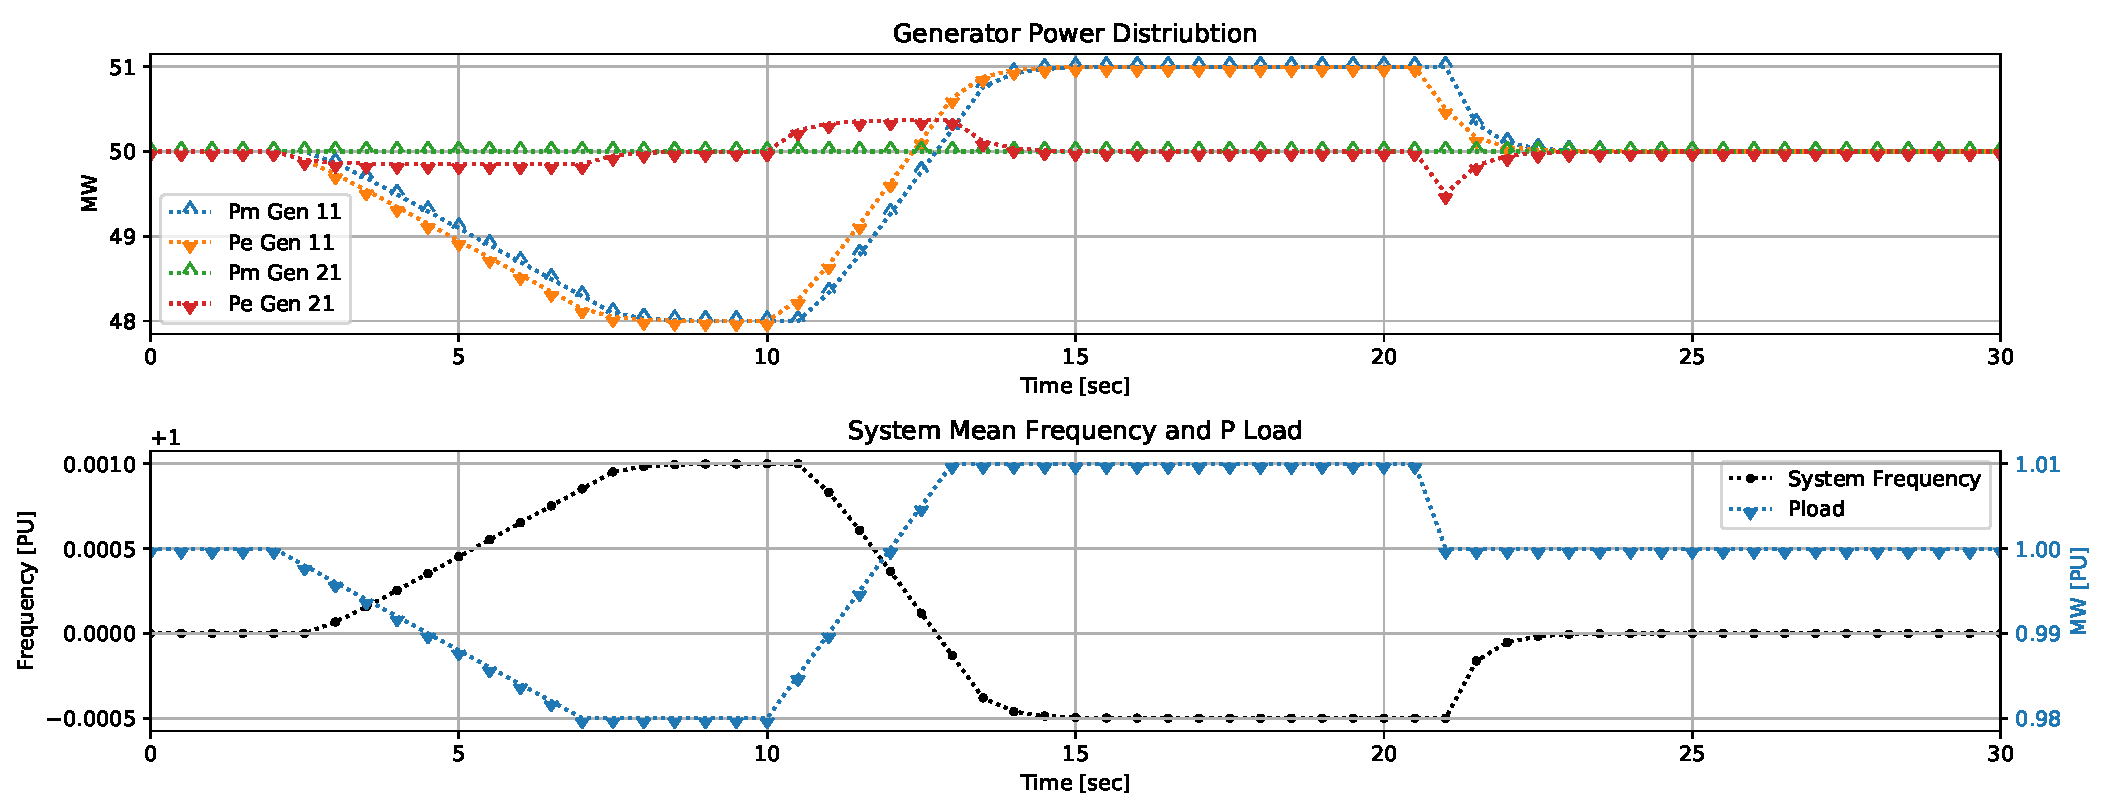
\includegraphics[width=\linewidth]{pythonRamp02}
\vspace{-1em}
\end{centering}
\vspace{-1em}
\paragraph{.ltd File Example:}
\begin{Verbatim}
# LTD simulation models / perturbances 
# Commented and empty lines are ignored during parsing.
# Double quoted variable names in model parameters also ignored

# pgov1  busnum busnam basekv id : #9 mwcap droop k1
#pgov1   21 "21" 22.00 "1 " : #9 mwcap=100.0 "droop" 0.05 "k1" 1.0
pgov1   11 "11" 22.00 "1 " : #9 mwcap=100.0 0.05 1.0

# Perturbances
# target bus id(optional) : pertType attribute time val abs(optional)
load 3 : "pertType" step  "pertTarget" p "startTime" 21 "newVal" -1 rel
load 3 : "pertType" ramp "pertTarget" p "startTime" 2 "RAtime" 5 "RAval" -2 "holdtime" 3 "RBtime" 3 "RBval" 3
\end{Verbatim}
\end{landscape}

 	place for comments

	\end{comment}
\end{document}